% A FAIRE
% Lier au thème de la ville
% Enoncer un but
% Montrer exemples (1 à 2) -> motivation
% Enoncer limitations (théo Rice -> côté ENS faire la preuve). Donc impossible de le vérifier à coup sûr dans le cas général.
% Solution: interprétation abstraite. Présentation vite fait de quelques moyens existant sur les strings.
% Moi, je fais mon propre "domaine d'interprétation abstrait": les automates.
% Explication rapide de comment ça se passe (on récupère l'ens. des états possibles au fur et à mesure puis inclus dans auto de ref).
% Je voulais le faire sur les grammaires, mais pb d'inclusion d'une grammaire dans un autre -> indécidable. Donc limité automates.

% 1ère partie: mise en place des outils.
% structure de représentation choisie (en OCAML): a = {...}, hashmap de transition. J'ai créé une lib entière pour.
% on peut donc construire toutes les opérations usuelles des automates là-dessus (union, inters, concat)
% ensuite, on crée un petit langage sur lequel je peux lancer tout ça.
% On se limite à 3 primitives pour simplifier: assignation string, concat, input utilisateur.
% On présente ici 2 quelques manières par lesquelles on construit l'automate: assignation directe, if/else, while.

% 2ème partie: application du modèle.
% On fait dérouler un programme en direct pour le montrer en application. (AST / prog clair / graphviz à chaque étape)
% On remarque qu'alors on arrive à montrer les modulo 3 et autres exemples d'applications.
% Screenshot du code qui marche.

% Dernière partie: Amélioration du modèle.
% Motivation: exemple du 2^n états des if/else consécutifs.
% On se concentre alors sur la réduction. D'ABORD JE FAIS LES TRUCS AVANT HEIN
% Résultats: mémoire + temps d'exec pour bcp bcp de if/else avec/sans réduction. Établir limite à laquelle c'est utile.
% Showcase de 2eme algo pour comparer. Tableaux récapitulatifs. (même diagramme évolution ?)
% Profiler pour voir quelles fonctions sont les + coûteuses...

% CCL pk pas des grammaires/automates à piles ? Pcq inclusion indécidable.
% Annexe preuve th. de Rice, preuve algo de brzozowski.


\documentclass{beamer}
\usepackage{listings}
\usepackage{amsmath}
\usepackage{bm}
\usepackage[font=small,labelfont=bf]{caption}
\usepackage{graphicx}
\graphicspath{ {./images/} }

\usetheme{Madrid}

%Information inclue dans la page de présentation
\title[Correction automatique de strings]{Vérification automatique de la correction de strings formés dynamiquement}
\subtitle{TIPE}
\author{Maire Grégoire}
\date{2023}

\newcommand{\prog}[1]{{\langle #1 \rangle}} 


% Met la table des matières au début de chaque section
\AtBeginSection[]
{
  \begin{frame}{Table des matières}
    \tableofcontents[currentsection]
  \end{frame}
}


%--------------------------------------------------------------
% Début du document
\begin{document}

\frame{\titlepage}

\begin{frame}{Motivations}
  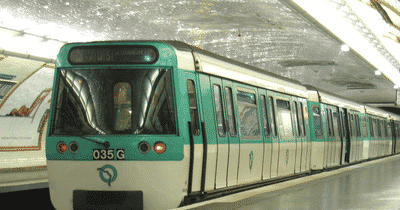
\includegraphics{ img_metro }
  \begin{itemize}
    \item En ville, les métros, voiture, avions ou autres transports en commun
      nécessitent l'assurance que leurs programmes soient corrects
    \item Longs programmes : besoin de preuves automatisées
    \item Mon but: automatiser les preuves d'invariants sur les strings dans les programmes
  \end{itemize}
\end{frame}

\begin{frame}{Motivations}
  \begin{itemize}
    \item Plus précisément, mon intérêt : construction dynamique d'un string dans un programme.
    \item Exemple d'application: Vérification d'un message formatté d'un métro à une unité de contrôle
  \end{itemize}
\end{frame}

\begin{frame}{Limitation}
  Ce qu'on aurait envie de faire : récolter l'ensemble des états possibles d'un string
  à la fin du code d'un programme. Mais ce n'est pas toujours possible :
  \begin{alertblock}{Limitation : Théorème de Rice [2]}
  Toute propriété sémantique non triviale d'un programme est indécidable (impossible à vérifier automatiquement).
  \end{alertblock}
  \begin{itemize}
    \item D'où l'utilisation d'une méthode pour contourner la limitation :
      \emph{l'interprétation abstraite}, consistant en une sur-approximation des états possibles d'arrivée.
    \item Il est toujours possible de sur-approximer (pas indécidable).
    \item Peut mener à des faux-négatifs, mais jamais à des faux-positifs. Mathématiquement correct !
  \end{itemize}
\end{frame}

\begin{frame}{Interpétation abstraite}
  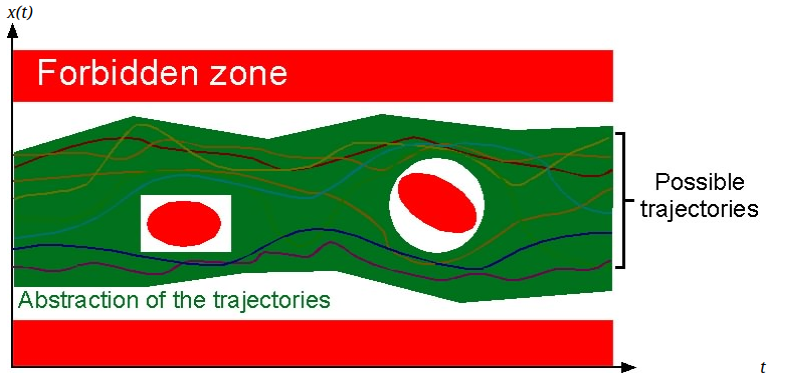
\includegraphics[scale=0.6]{ absint_nutshell }
  \captionof{figure}{Visualisation de l'interprétation abstraite [1]}
\end{frame}

\begin{frame}{Choix d'un domaine abstrait}
  Pour ce faire, on définit un \emph{domaine abstrait} pour
  représenter l'ensemble des valeurs prises par le string
  
  Domaines déjà existants:
  \begin{itemize}
    \item Domaine sur les préfixes : "l'ensemble de tous les strings commençant par..."
    \item Domaine sur les facteurs communs: "l'ensemble de tous les strings ayant comme facteur..."
  \end{itemize}
  
  Création d'un domaine inexploré: la représentation par automates.
  \begin{itemize}
    \item[\textcolor{green}{\textbullet}] Précis
    \item[\textcolor{red}{\textbullet}] Plus coûteux
  \end{itemize}
\end{frame}

\begin{frame}{Un exemple concret}
  \begin{center}
  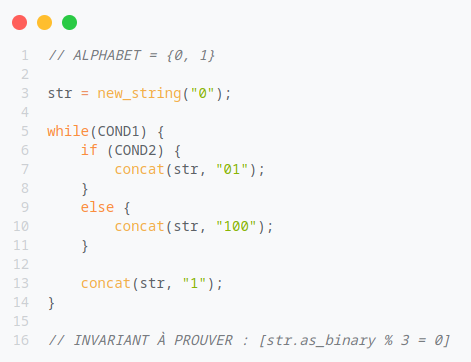
\includegraphics[scale=0.7]{ prog0 }
  \captionof{figure}{Un programme construisant des nombres congru à 0 modulo 3}
  Prouvons sa correction automatiquement !
  \end{center}
\end{frame}

\begin{frame}{Table des matières}
  \tableofcontents
\end{frame}


\section{Implémentation des outils}

\begin{frame}{Structure d'automates}
  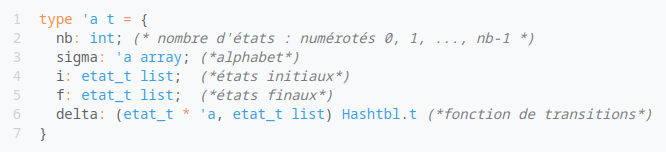
\includegraphics[scale=0.7]{ type_automate }
  \captionof{figure}{Structure choisie pour représenter les automates}
  \begin{itemize}
    \item Affichage (par Graphviz)
    \item Acceptation d'un mot
    \item Complété, Émondé, Déterminisé, Complémentaire
    \item Union, Intersection.
  \end{itemize}
\end{frame}


\begin{frame}{Langage de test}
  On considère un string en particulier qu'on construit.
  
  Pour appliquer la théorie, création d'un mini-langage, avec certaines primitives de string intégrées.
  
  Syntaxe (inductive) du langage:

  \begin{minipage}{1.5in}
    \begin{align*}
      stat &:= stat\; \mathbf{;}\; stat \\
      &\;|\; \mathbf{if}\; cond\; \mathbf{then}\; stat\; \mathbf{else}\; stat \\
      &\;|\; \mathbf{while}\; cond\; \mathbf{do}\; stat\; \mathbf{done} \\
      &\;|\; \mathbf{skip} \\
      &\;|\; \mathbf{assert}(cond) \\
      &\;|\; stringop
    \end{align*}
  \end{minipage}
  \begin{minipage}{2.5in}
    \begin{align*}
      cond &:= \mathbf{unknown} \\
      &\;|\; b \in Bool \\
      &\;|\; \mathbf{not}\; cond \\
      &\;|\; cond \wedge cond \\
      &\;|\; cond \vee cond \\
    \end{align*}
  \end{minipage}
  \begin{minipage}{1.5in}
    \begin{align*}
      stringop &:=  \mathbf{new\_string}(str) \\
      &\;|\; \mathbf{push\_left}(str) \\
      &\;|\; \mathbf{push\_right}(str)
    \end{align*}
  \end{minipage}
\end{frame}

\begin{frame}{Le langage en pratique}
  \begin{itemize}
    \item En pratique, seulement un AST
      mais je présenterai les exemples en code directement.
    \item Le programme d'introduction peut ainsi être représenté de la sorte:
  \end{itemize}
  \begin{center}
    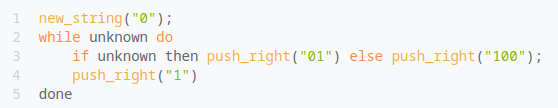
\includegraphics[width=\linewidth]{ prog1 }
    \captionof{figure}{Programme d'introduction avec la syntaxe créée}
  \end{center}
\end{frame}

\begin{frame}{Sémantique de récolte des états}
  \begin{itemize}
  \item But: récolter l'ensemble des états possibles du string au fur et à mesure du programme
  \item Concept : récolte séquentielle des états par une fonction de transfert pour amener à l'étape suivante de l'algorithme
  % TODO illustrer mieux ce que je veux dire ici... par l'exemple du "if" on fait un bô dessin
  \end{itemize}

\end{frame}

\begin{frame}{Cas du while}
  Un cas ardu se pose : la récolte d'états après un $while$.

  Lorsqu'on arrive sur un while, on effectue les procédures suivantes :
  \begin{itemize}
    \item Récolte de l'intégralité des opérations sur le string dans le while
    \item S'il ne contient que des \texttt{push\_right}, alors on ajoute une boucle à l'automate. (point fixe des états)
  \end{itemize}
\end{frame}

\begin{frame}
  \begin{center}
  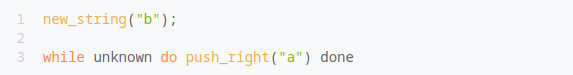
\includegraphics[width=0.8\linewidth]{ while0 }
  \captionof{figure}{Code d'exemple}
    \begin{minipage}{0.48\linewidth}
      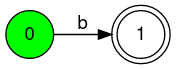
\includegraphics[width=0.45\linewidth]{ while1 }
      \captionof{figure}{Après 0 entrée dans le while}
    \end{minipage}
    \hfill
    \begin{minipage}{0.49\linewidth}
      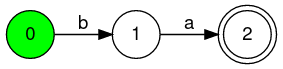
\includegraphics[width=0.7\linewidth]{ while2 }
      \captionof{figure}{Après 1 entrée dans le while}
    \end{minipage}

    \begin{minipage}{0.48\linewidth}
      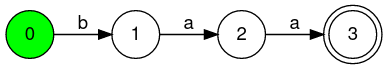
\includegraphics[width=0.9\linewidth]{ while3 }
      \captionof{figure}{Après 2 entrées dans le while}
    \end{minipage}
    \hfill
    \begin{minipage}{0.48\linewidth}
      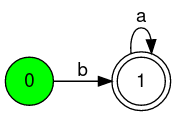
\includegraphics[width=0.45\linewidth]{ while4 }
      \captionof{figure}{Approximation du point fixe du while}
    \end{minipage}
    Approximation \emph{correcte} car on récupère au moins les états accessibles.
  \end{center}
\end{frame}


\section{Appplication}

\begin{frame}{Application 1 : modulo 3}
  Application sur le programme d'introduction :

  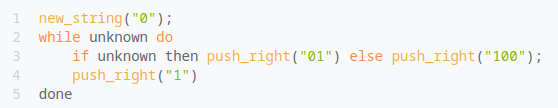
\includegraphics[scale=0.6]{ prog1 }

  \begin{minipage}{0.49\linewidth}
    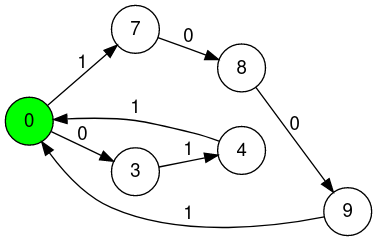
\includegraphics[width=\linewidth]{ application1 }
    \captionof{figure}{Automate généré}
  \end{minipage}%
  \hfill
  \begin{minipage}{0.40\linewidth}
    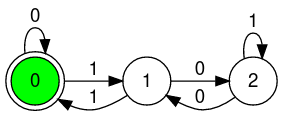
\includegraphics[width=\linewidth]{ mod_3_ref }
    \captionof{figure}{Automate de référence}
  \end{minipage}
  % TODO faire un petit dessin d'inclusion :heart_eyes:
  On vérifie automatiquement que le langage de l'automate généré est inclus dans celui
  de l'automate de référence.
\end{frame}


\section{Améliorations diverses}

\begin{frame}{Explosion d'états}
  Considérons le programme suivant :
  \begin{center}
    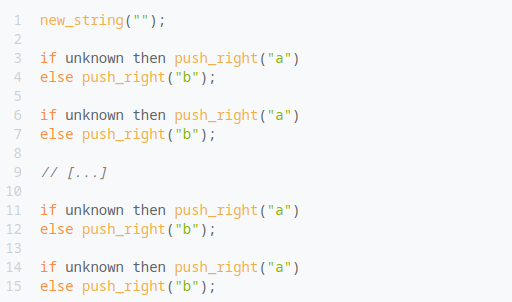
\includegraphics[width=0.7\linewidth]{ expl0 }
  \end{center}
\end{frame}

\begin{frame}{Explosion d'états} % comparer 2 approches (déterminiser à l'avance, ou non) + graphiques comparatif
  Explosion exponentielle des états par rapport au nombre de \texttt{if}:
  
  \begin{minipage}{0.49\linewidth}
    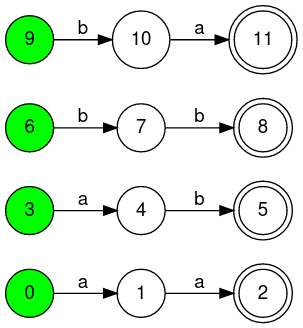
\includegraphics[width=0.8\linewidth]{ expl1 }
    \captionof{figure}{Automate généré pour 2 \texttt{if} successifs}
  \end{minipage}
  \hfill
  \begin{minipage}{0.4\linewidth}
    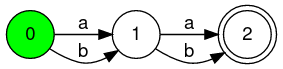
\includegraphics[width=\linewidth]{ expl2 }
    \captionof{figure}{Un autre automate reconnaissant le même langage}
  \end{minipage}
\end{frame}


\begin{frame}{Solution à l'explosion d'états}
  \begin{itemize}
    \item Solution possible: minimisation de l'automate
  \end{itemize}
    \begin{alertblock}{Algorithme de Brzozowski [3]}
      On pose $t(\mathcal{A})$ l'automate transposé de $\mathcal{A}$, $d(\mathcal{A})$ le déterminisé de $\mathcal{A}$.
      
      Alors : $\mathcal{A}' = d(t(d(t(\mathcal{A}))))$ est l'automate minimal de $\mathcal{A}$.
    \end{alertblock}
\end{frame}

\begin{frame}
  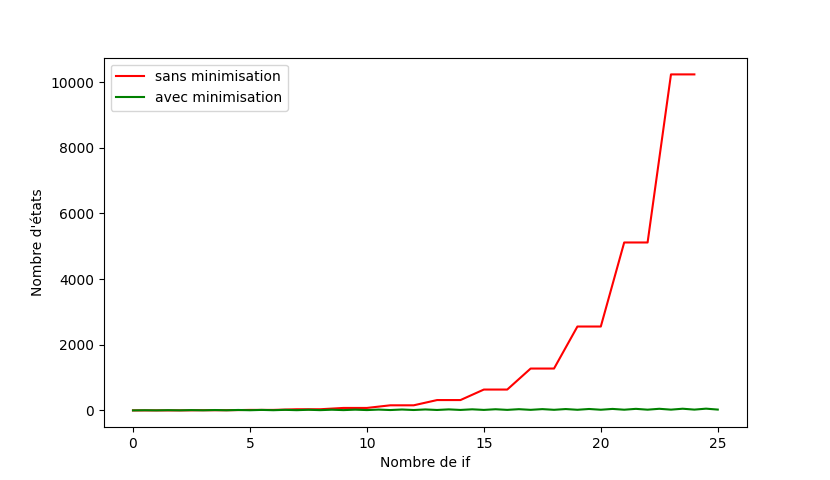
\includegraphics[scale=0.6]{ graphique_etats }
  \captionof{figure}{Evolution du nombre d'états en fonction du nombre de if}
\end{frame}

\section{Conclusion}

\begin{frame}{Conclusion}
  \begin{itemize}
    \item Construction d'un nouveau domaine abstrait
    \item Application sur certains programmes
    \item Mise en évidence et amélioration de certaines limitations
  \end{itemize}
\end{frame}


\section{Annexe}

\begin{frame}{Annexe: Preuve du Théorème de Rice [2]}
  \begin{alertblock}{Énoncé du théorème}
    Soit f une fonction booléenne totale prenant en entrée un algorithme, telle que
    f est non-triviale, et f conserve l'équivalence sémantique.

    Alors f est non-calculable.
  \end{alertblock}
  Soient $\prog{F} = \prog{\texttt{while (true)}}$.
  et $\prog{B}$ tel que $f(\prog{B}) \neq f(\prog{F})$

  On pose $tr$: $(\prog{A},e) \longmapsto \prog{x \mapsto A(e); B(x)}$

  Soient $A$ un algorithme et $e$ une entrée de $A$.

  \underline{Si $A(e)$ finit:} $tr(A, e)$ $\sim$ $\prog{B}$ donc $f(tr(\prog{A}, e)) = f(\prog{B})$
  
  \underline{Sinon:} $tr(\prog{A}, e) \sim \prog{F}$ donc $f(tr(\prog{A}, e)) = f(\prog{F})$

  \underline{Ainsi:}
  \begin{align*}
    f(tr(\prog{A}, e)) = f(\prog{B}) & \Longleftrightarrow A(e) \text{ termine} \\
                                     & \Longleftrightarrow Arret(\prog{A}, e)
  \end{align*}

  D'où une réduction du problème $Arret$ (resp. $\neg Arret$).
\end{frame}

\begin{frame}{Annexe: Preuve de la correction de minimisation}
  \begin{alertblock}{Algorithme de Brzozowski [3]}
    On pose $t(\mathcal{A})$ l'automate transposé de $\mathcal{A}$, $d(\mathcal{A})$ le déterminisé par parties de $\mathcal{A}$
    obtenu en ne gardant que les états accessibles.
    
    Alors on a : $\mathcal{A}' = d(t(d(t(\mathcal{A}))))$ est l'automate minimal de $\mathcal{A}$.
  \end{alertblock}
  Cet automate reconnaît le même langage que $\mathcal{A}$ sans soucis.
  
  Soient $P$ et $P'$ deux états distincts de $\mathcal{A}'$.



  
  Par définition, $P$ et $P'$ sont deux ensembles-états de l'automate $d(t(\mathcal{A}))$.
  Soit $R$ un état de $d(t(\mathcal{A}))$, tel que $R \in P$ et $R \notin P'$. $R$ est aussi un ensemble-état, qui vérifie,
  par définition du transposé, $R = \{q \;|\; q \xrightarrow{w} f \text{ dans } \mathcal{A} \text{, avec } f \in F\}$ pour un certain mot $w$.
  On en déduit que dans $\mathcal{A'}$, il existe un chemin étiquetté par $w$ vers un état final,
  alors que ce n'est pas le cas pour $P'$. Donc $P$ et $P'$ ne sont pas des états équivalents. % TODO reformuler
\end{frame}

\begin{frame}{Bibliographie}
  \begin{itemize}
    \item [1] Visualisation de l'interprétation abstraite:
    https://www.di.ens.fr/~cousot/AI/IntroAbsInt.html
    \item [2] Théorème de Rice: H. G. Rice, Classes of Recursively Enumerable Sets
    and Their Decision Problems, Transactions of the American Mathematical
    Society, volume 74, numéro 2, mars 1953
    \item [3] Algorithme de Brzozowski :Janusz A. Brzozowski, \emph{Canonical regular
    expressions and minimal state graphs for definite events}, Proceedings of the
    Symposium on Mathematical Theory of Automata, Polytechnic Institute of Brooklyn,
    April 1962, New York, Wiley, 1963, p. 529-561
    \item [4] Domaines de strings existant:
    https://pm.inf.ethz.ch/publications/CostantiniFerraraCortesi11.pdf
  \end{itemize}
\end{frame}

\end{document}


% TODO ENS: faire rapport.
% TODO ENS: rajouter code 
% TODO ENS: mettre le code en annexe(en imprimé d'ailleurs). 